\documentclass[12pt]{article}

% --- Packages ---
\usepackage[utf8]{inputenc}
\usepackage[T1]{fontenc}
\usepackage[french]{babel}
\usepackage{amsmath, amssymb}
\usepackage{geometry}
% \usepackage[draft]{graphicx}
\usepackage{tikz}
\usepackage[most]{tcolorbox}
\usepackage{multicol}
\usepackage{lmodern}
\usepackage{pgfplots}
\pgfplotsset{compat=1.18}
\usepackage{mdframed}
\usepackage{tkz-tab}
\usepackage{bm}
\usepackage{xcolor}
\usepackage{sectsty}
\usepackage[utf8]{inputenc}
\usepackage[T1]{fontenc}
\usepackage[inline]{enumitem}
\usepackage[dvipsnames]{xcolor}
\usepackage{multido}
% --- Page ---
\geometry{margin=2cm}

% Footer
\usepackage{fancyhdr}
\pagestyle{fancy}
\cfoot{\thepage}
\rfoot{\textit{G.M.}}
\renewcommand{\headrulewidth}{0pt}
\renewcommand{\footrulewidth}{0pt}

% Pour les normes : 
\newcommand*{\norme}[1]{\left\lVert\overrightarrow{#1}\right\rVert}

\usetikzlibrary{shapes.misc}

\tikzset{cross/.style={cross out, draw=black, minimum size=2*(#1-\pgflinewidth), inner sep=0pt, outer sep=0pt},
%default radius will be 1pt. 
cross/.default={4pt}}

% mettre dans le préambule, après \usepackage{xcolor}
\usepackage{sectsty} % gère facilement la couleur des titres
\setlength{\parindent}{0pt}

\sectionfont{\color{red}\Large\bfseries}     % pour \section*
\subsectionfont{\color{red}\large\bfseries\hspace{1cm}}

\begin{document}

% ============================
%   Informations chiffrées
% ============================

\newpage

\begin{center}
    {\LARGE \textbf{Informations chiffrées}}\\[4mm]
    {\large Seconde}
\end{center}

\hrule
\vspace{0pt}

% ============================
%   PARTIE 1 : Proportions et pourcentages
% ============================

\section*{\textcolor{red}{Partie 1 : Proportions et pourcentages}}

\subsection*{\hspace{1cm} 1) Proportions et pourcentages}

\vspace{5pt}
\underline{{\color{ForestGreen}\bf{Définition exemple :}}}

\begin{minipage}[t]{.45\textwidth}%
    \vspace{0pt}
    La population totale des élèves de 2nde
    
    \vspace{10pt}
    
    compte \_\_\_\_\_\_\_\_ élèves.
    
    \vspace{10pt}
    
    C’est la population de \textbf{référence}.

    \vspace{10pt}
    
    La sous-population des élèves externes 
    
    \vspace{10pt}
    
    compte \_\_\_\_\_\_\_\_ élèves.

    \vspace{20pt}
    \hspace{0.5cm} \textbf{a)} La proportion d’élèves externes parmi tous les élèves de 2nde est : 

    \[
    p = \ \ \ \ \ \ \ \ \ \ \ \ \ \ \ \ \ \ \ \ 
    \]

    \vspace{10pt}
    Cette proportion peut s'exprimer en pourcentage : 

    \[
    p = \ \ \ \ \ \ \ \ \ \ \ \ \ \ \ \ \ \ \ \ 
    \]
\end{minipage}%
\hfill
\begin{minipage}[t]{.45\textwidth}%
    \vspace{40pt}
    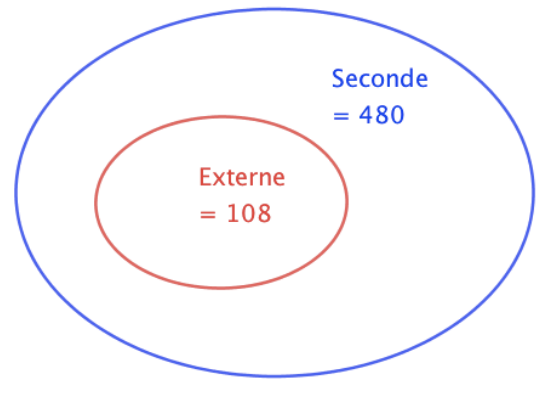
\includegraphics[width=1\textwidth]{exemple1.png}
\end{minipage}%

\vspace{20pt}

\hspace{0.5cm} \textbf{b)} Parmi les 480 élèves de 2nde, 15\% ont choisi l’option grec, soit : 

\vspace{4cm}

\begin{mdframed}[
    linewidth=1pt,
    linecolor=RoyalBlue,
    innertopmargin=10pt,
    innerbottommargin=10pt
]
{\color{RoyalBlue}\textbf{\underline{Exercice d'application n°1 :} 
Travailler avec les proportions et pourcentages}}
\vspace{10pt}

Une société de 75 employés compte 12\% de cadres et le reste d’ouvriers.
35 employés de cette société sont des femmes et 5 d’entre elles sont cadres.

\hspace{1cm} a) Calculer l’effectif des cadres.

\hspace{1cm} b) Calculer la proportion de femmes dans cette société.

\newpage
\hspace{1cm} c) Calculer la proportion, en \%, de cadres parmi les femmes.

\hspace{1.5cm} Y a-t-il plus de femmes cadres ou d'hommes cadres dans cette société ?

\vspace{0.5cm}
{\color{black!27}\dotfill}

\vspace{0.5cm}
{\color{black!27}\dotfill}

\vspace{0.5cm}
{\color{black!27}\dotfill}

\vspace{0.5cm}
{\color{black!27}\dotfill}

\vspace{0.5cm}
{\color{black!27}\dotfill}

\end{mdframed}


\vspace{10pt}

% ========================================================
%             2) Pourcentage de pourcentage
% ========================================================
\subsection*{\hspace{1cm} 2) Pourcentage de pourcentage}

\vspace{5pt}
\underline{{\color{ForestGreen}\bf{Définition exemple :}}}

\begin{minipage}[t]{.4\textwidth}%
    \vspace{0pt}
    Dans un bus, il y a 40\% de scolaires.
    
    Et parmi les scolaires, 60\% sont des filles.

    \vspace{10pt}
    
    La proportion de scolaires filles dans le bus est donc égale à : 

    \vspace{4cm}
\end{minipage}%
\hfill
\begin{minipage}[t]{.55\textwidth}%
    \vspace{20pt}
    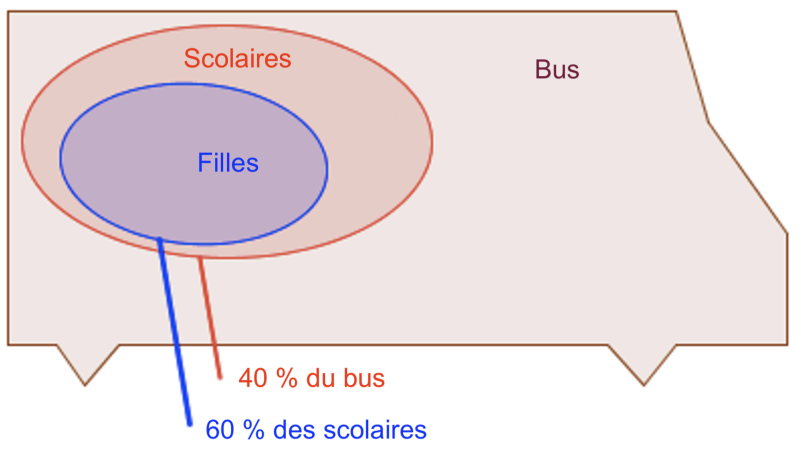
\includegraphics[width=1\textwidth]{exemple2.png}
\end{minipage}%

\begin{mdframed}[
    linewidth=1pt,
    roundcorner=5pt,
    linecolor=Red,
    innertopmargin=10pt,
    innerbottommargin=10pt
]
{\color{red}
\underline{Propriété :}}

\vspace{5pt}
\begin{minipage}[t]{.45\textwidth}%
    \vspace{0pt}
    Soient $A \subset B$ et $B \subset C$.

    \vspace{10pt}
    
    {\color{blue}Soit $p_1$ la proportion de $A$ dans $B$.}

    \vspace{10pt}
    
    {\color{red}Soit $p_2$ la proportion de $B$ dans $C$.}
\end{minipage}%
\hfill
\begin{minipage}[t]{.45\textwidth}%
    \vspace{-25pt}
    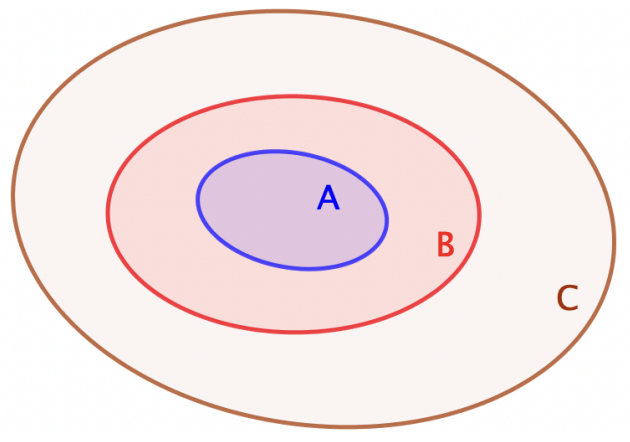
\includegraphics[width=0.7\textwidth]{prop1.png}
\end{minipage}%

\vspace{-5pt}
\begin{center}
    Alors {\color{blue}$p_1$} $\times$ {\color{red}$p_2$} est la proportion de 
    $A$ dans $C$.
\end{center}
\end{mdframed}

\vspace{5pt}

\underline{Remarque :} Pour calculer un pourcentage de pourcentage, on \textbf{multiplie} les pourcentages entre eux.

\vspace{5pt}

\begin{center}
    {\color{red}\underline{\textbf{À RETENIR :}}} Toujours s'aider d'un 
    \textbf{schéma représentatif} de la situation.    
\end{center}

\vspace{10pt}

\begin{mdframed}[
    linewidth=1pt,
    linecolor=RoyalBlue,
    innertopmargin=10pt,
    innerbottommargin=10pt
]
{\color{RoyalBlue}\textbf{\underline{Exercice d'application n°2 :} Calculer un 
pourcentage de pourcentage.}}
\vspace{5pt}

Sur 67 millions d’habitants en France, 66\% de la population est en âge de travailler (15-64 ans).

\vspace{5pt}

La population active représente 70\% de la population en âge de travailler.

\vspace{5pt}

a) Calculer la proportion de population active par rapport à la population totale.

\vspace{5pt}

b) Combien de français compte la population active ?

\vspace{0.5cm}
{\color{black!30}\dotfill}

\vspace{0.5cm}
{\color{black!30}\dotfill}

\vspace{0.5cm}
{\color{black!30}\dotfill}

\vspace{0.5cm}
{\color{black!30}\dotfill}

\vspace{0.5cm}
{\color{black!30}\dotfill}

\vspace{0.5cm}
{\color{black!30}\dotfill}

\vspace{20pt}

\end{mdframed}

\vspace{20pt}

% ========================================================
%             Partie 2 : Évolutions
% ========================================================
\section*{\textcolor{red}{Partie 2 : Évolutions}}

% ========================================================
%             1) Taux d'évolution
% ========================================================
\subsection*{\hspace{1cm} 1) Taux d'évolution}

\begin{mdframed}[
    linewidth=1pt,
    linecolor=ForestGreen,
    innertopmargin=10pt,
    innerbottommargin=10pt
]
{\color{ForestGreen}\textbf{\underline{Définition :}}}  

On considère une valeur initiale $V_I$ qui subit une évolution pour arriver à une valeur finale $V_F$.

Le taux d'évolution est alors égal à :
\[
t = \dfrac{V_F-V_I}{V_I}
\]

\end{mdframed}

\underline{Remarque :}
\begin{itemize}
    \item Si $\bm{t>0}$, l'évolution est une \textbf{augmentation}
    \item Si $\bm{t<0}$, l'évolution est une \textbf{diminution}
\end{itemize}

\begin{mdframed}[
    linewidth=1pt,
    linecolor=RoyalBlue,
    innertopmargin=10pt,
    innerbottommargin=10pt
]
{\color{RoyalBlue}\textbf{\underline{Exercice d'application n°3 :}
Calculer un taux d'évolution.}}

\vspace{5pt}
La population d'un village est passé de 8500 à 10400 entre 2018 et 2022.
Calculer le taux d'évolution de la population en \%.

\vspace{0.5cm}
{\color{black!30}\dotfill}

\vspace{0.5cm}
{\color{black!30}\dotfill}

\vspace{0.5cm}
{\color{black!30}\dotfill}

\vspace{0.5cm}
{\color{black!30}\dotfill}

\end{mdframed}

\vspace{20pt}


% ========================================================
%             2) Coefficient multiplicateur
% ========================================================
\subsection*{\hspace{1cm} 2) Coefficient multiplicateur}

\vspace{5pt}
\begin{mdframed}[
    linewidth=1pt,
    roundcorner=5pt,
    linecolor=Red,
    innertopmargin=10pt,
    innerbottommargin=10pt
]
{\color{red}
\underline{Propriété :}

\vspace{5pt}
Augmenter un nombre de t\% revient à le \textbf{multiplier} par $1 + \dfrac{t}{100}$.

\vspace{5pt}
Diminuer un nombre de t\% revient à le \textbf{multiplier} par $1 - \dfrac{t}{100}$.

\vspace{5pt}
\begin{minipage}[t]{.45\textwidth}%
    \vspace{0pt}
    \hspace{3cm}
    $
    \left\{
        \begin{array}{ll}
            1 + \dfrac{t}{100}, & \mbox{\bf{si $\bm{\nearrow}$}} \\
            \ \\
            1 - \dfrac{t}{100}, & \mbox{\bf{si $\bm{\searrow}$}}
        \end{array}
    \right.
    $
\end{minipage}%
\hfill
\begin{minipage}[t]{.55\textwidth}%
    \vspace{15pt}
    Ces nombres sont appelés 
    
    \textbf{coefficients multiplicateurs}
\end{minipage}%
}
\end{mdframed}

\vspace{5pt}
\underline{Exemples :}

\begin{center}
    \def\arraystretch{3}
    \begin{tabular}{|c|p{8cm}|}
        \hline
        Taux d'évolution & Coefficient multiplicateur \\
        \hline
        +38\% & $1+\dfrac{38}{100} = 1 + 0,38 = 1,38$ \\[8pt]
        \hline
        -45\% & $1-\dfrac{45}{100} = 1 - 0,45 = 0,55$ \\[8pt]
        \hline
        +5\% & \ \ \ \ \ \ \ \ \ \ \ \  \\[40pt]
        \hline
        -4\% & \ \ \ \ \ \ \ \ \ \ \ \  \\[40pt]
        \hline
    \end{tabular}
\end{center}

\begin{mdframed}[
    linewidth=1pt,
    linecolor=RoyalBlue,
    innertopmargin=10pt,
    innerbottommargin=10pt
]
{\color{RoyalBlue}\textbf{\underline{Exercice d'application n°4 :}
Calculer un nombre après une augmentation ou diminution en pourcentage.}}

\vspace{5pt}
\hspace{1cm} a) Le prix d'un blouson qui coutait 160 € est réduit de 35 %.

\hspace{1.5cm} Calculer le nouveau prix du blouson.

\hspace{1cm} b) Le prix d'un survêtement qui coûtait 49 € est augmenté de 8 %.

\hspace{1.5cm} Calculer le nouveau prix du survêtement.

\vspace{0.5cm}
{\color{black!30}\dotfill}

\vspace{0.5cm}
{\color{black!30}\dotfill}

\vspace{0.5cm}
{\color{black!30}\dotfill}

\vspace{0.5cm}
{\color{black!30}\dotfill}

\vspace{0.5cm}
{\color{black!30}\dotfill}

\vspace{0.5cm}
{\color{black!30}\dotfill}

\vspace{0.5cm}
{\color{black!30}\dotfill}

\vspace{0.5cm}
{\color{black!30}\dotfill}

\vspace{0.5cm}
{\color{black!30}\dotfill}

\end{mdframed}



\vspace{20pt}


% ========================================================
%             Partie 3 : Évolutions successives, évolutions réciproques
% ========================================================
\section*{\textcolor{red}{Partie 3 : Évolutions successives, évolution réciproque}}

% ========================================================
%             1) Évolutions successives
% ========================================================
\subsection*{\hspace{1cm} 1) Évolutions successives}

\vspace{5pt}
\underline{{\color{ForestGreen}\bf{Définition exemple :}}}

\vspace{5pt}
On augmente un prix de 5\%, puis on l’augmente à nouveau de 20\%.

On a effectué deux
évolutions successives.

\vspace{5pt}
\textbf{{\color{red}\underline{Attention :}}} +5\% suivi de +20\% n’équivaut pas à +25\% !

\vspace{5pt}
Pour calculer le taux d’évolution global, on fait :

\vspace{10pt}

\vspace{0.5cm}
{\color{black!30}\dotfill}

\newpage
\begin{mdframed}[
    linewidth=1pt,
    roundcorner=5pt,
    linecolor=Red,
    innertopmargin=10pt,
    innerbottommargin=0pt
]
{\color{red}
\underline{Propriété :}

\vspace{5pt}
Soient $CM_1$ et $CM_2$ deux coefficients multiplicateurs correspondants à deux évolutions
successives.

L'évolution finale correspond au coefficient multiplicateur : 
\[
CM = CM_1 \times CM_2
\]
}
\end{mdframed}

\begin{mdframed}[
    linewidth=1pt,
    linecolor=RoyalBlue,
    innertopmargin=10pt,
    innerbottommargin=10pt
]
{\color{RoyalBlue}\textbf{\underline{Exercice d'application n°5 :} 
Déterminer un taux d'évolution global}}
\vspace{10pt}

En 2021, la boulangerie-pâtisserie Aux délices a augmenté ses ventes de 10\%. En 2022, l'inflation a fait
diminuer ses ventes de 5\%.

\vspace{5pt}
Calculer le \textbf{taux d'évolution} global des ventes sur les deux années.

\vspace{0.5cm}
{\color{black!27}\dotfill}

\vspace{0.5cm}
{\color{black!27}\dotfill}

\vspace{0.5cm}
{\color{black!27}\dotfill}

\vspace{0.5cm}
{\color{black!27}\dotfill}

\vspace{0.5cm}
{\color{black!27}\dotfill}

\end{mdframed}





% ========================================================
%             2) Évolution réciproque
% ========================================================
\subsection*{\hspace{1cm} 2) Évolution réciproque}

\vspace{5pt}
\underline{{\color{ForestGreen}\bf{Définition exemple :}}}

\vspace{5pt}
On augmente un prix de 25\%. 

Puis on diminue ce prix pour qu’il retrouve le prix de départ.

Cette diminution s’appelle une \textbf{évolution réciproque}.

\vspace{5pt}
Pour calculer le taux d’évolution réciproque, on fait :

\vspace{10pt}

\vspace{0.5cm}
{\color{black!30}\dotfill}

\vspace{0.5cm}
{\color{black!30}\dotfill}

\vspace{0.5cm}
{\color{black!30}\dotfill}

\vspace{0.5cm}
{\color{black!30}\dotfill}

\newpage
\begin{mdframed}[
    linewidth=1pt,
    roundcorner=5pt,
    linecolor=Red,
    innertopmargin=10pt,
    innerbottommargin=0pt
]
{\color{red}
\underline{Propriété :}

\vspace{5pt}
Soit $CM$ le coefficient multiplicateur correspondant à une évolution.

\vspace{5pt}
L'évolution réciproque correspond au coefficient multiplicateur réciproque : 
\[
CM' = \dfrac{1}{CM}
\]
}
\end{mdframed}

\begin{mdframed}[
    linewidth=1pt,
    linecolor=RoyalBlue,
    innertopmargin=10pt,
    innerbottommargin=10pt
]
{\color{RoyalBlue}\textbf{\underline{Exercice d'application n°5 :} 
Déterminer un taux taux d'évolution réciproque.}}
\vspace{10pt}

\hspace{1cm} a) Un magasin a des ventes en diminution de 8\% sur l'année 2022.

\hspace{1.5cm} Quel devrait être le pourcentage d'évolution sur l'année 2023 pour que les ventes retrouvent
leur valeur initiale ?

\vspace{5pt}
\hspace{1cm} b) La population d’un village a augmenté de 3\% sur une année puis retrouve sa valeur initiale
l’année suivante.

\hspace{1.5cm} Quel est le pourcentage de baisse sur la 2\up{ème} année ?

\vspace{0.5cm}
{\color{black!27}\dotfill}

\vspace{0.5cm}
{\color{black!27}\dotfill}

\vspace{0.5cm}
{\color{black!27}\dotfill}

\vspace{0.5cm}
{\color{black!27}\dotfill}

\vspace{0.5cm}
{\color{black!27}\dotfill}

\vspace{0.5cm}
{\color{black!27}\dotfill}

\vspace{0.5cm}
{\color{black!27}\dotfill}

\vspace{0.5cm}
{\color{black!27}\dotfill}

\vspace{0.5cm}
{\color{black!27}\dotfill}

\vspace{0.5cm}
{\color{black!27}\dotfill}

\vspace{0.5cm}
{\color{black!27}\dotfill}

\vspace{0.5cm}
{\color{black!27}\dotfill}

\vspace{0.5cm}
{\color{black!27}\dotfill}

\vspace{20pt}

\end{mdframed}






\vspace{20pt}







\end{document}
